\label{ap:ap14}
\chapter{Visualização de dados e storytelling}
\section*{\textbf{A - ENUNCIADO}}

\textcolor[HTML]{1D2125}{Escolha um conjunto de dados brutos (ou uma visualização de dados que você acredite que possa
ser melhorada) e faça uma visualização desses dados (de acordo com os dados escolhidos e com a ferramenta de sua
escolha)}

\textcolor[HTML]{1D2125}{Desenvolva uma narrativa/storytelling para essa visualização de dados considerando os conceitos
e informações que foram discutidas nesta disciplina. Não esqueça de deixar claro para seu possível público alvo
qual }\textbf{\textcolor[HTML]{1D2125}{o objetivo dessa visualização de dados, o que esses dados significam, quais
possíveis ações podem ser feitas com base neles.}}\textcolor[HTML]{1D2125}{ }

\textbf{\textcolor[HTML]{1D2125}{Entregue em um PDF:}}

\textcolor[HTML]{1D2125}{{}- O }\textbf{\textcolor[HTML]{1D2125}{conjunto de dados
brutos}}\textcolor[HTML]{1D2125}{ (}\textbf{\textcolor[HTML]{1D2125}{ou uma visualização de
dados }}\textcolor[HTML]{1D2125}{que você acredite que possa
ser }\textbf{\textcolor[HTML]{1D2125}{melhorada}}\textcolor[HTML]{1D2125}{);}

\textcolor[HTML]{1D2125}{{}- Explicação do }\textbf{\textcolor[HTML]{1D2125}{contexto e o
publico-alvo}}\textcolor[HTML]{1D2125}{ da visualização de dados e do storytelling que será desenvolvido;}

\textcolor[HTML]{1D2125}{{}- A }\textbf{\textcolor[HTML]{1D2125}{visualização desses
dados}}\textcolor[HTML]{1D2125}{ (de acordo com os dados escolhidos e com a ferramenta de sua
escolha) }\textbf{\textcolor[HTML]{1D2125}{explicando a escolha do tipo de visualização e da ferramenta
usada}}\textcolor[HTML]{1D2125}{; (}\textbf{\textcolor[HTML]{1D2125}{50 pontos}}\textcolor[HTML]{1D2125}{)}



%%%%%%%%%%%%%%%%%%%%%%%%%%%%%%%%%%%%%%%%%%%%%%%%%%%%%%%%%%%%%%%%%%%%%%%%%%%%%%%%%%%%%%%%%%%%%
\section*{\textbf{B - RESOLUÇÃO}}
\subsection*{\textbf{Titulo}}
\noindent A Revolução de Stephen Curry no Basquete Moderno


\subsection*{\textbf{Contexto e Público-Alvo}}
Stephen Curry revolucionou o basquete com sua habilidade nos arremessos de 3 pontos. Desde que entrou
na NBA em 2009, ele não apenas quebrou recordes, mas também mudou a forma como o jogo é jogado,
tornando os arremessos de longa distância uma parte essencial das estratégias ofensivas.

Esta visualização de dados tem como objetivo mostrar o impacto de Curry, analisando suas tentativas,
acertos e porcentagem de conversão de arremessos de 3 pontos por temporada.

O público-alvo inclui:
\begin{itemize}
    \item Fãs de basquete, que querem entender a revolução do jogador.
    \item Estudantes de estatística, interessados em analisar como os números traduzem a influência de um
atleta.
    \item Analistas esportivos e treinadores, que podem usar essas informações para comparar Curry com
outros jogadores e entender como o jogo evoluiu.
\end{itemize}

\subsection*{\textbf{Descrição da Narrativa/Storytelling}}
Esta análise se baseia em apresentar a jornada de Stephen Curry e sua evolução como um arremessador de
3 pontos. As ferramentas utilizadas para geração do mesmo foram Python com auxílio das bibliotecas
Matplotlib e Seaborn. Os dados foram extraídos do portal \url{https://www.basketball-reference.com/} que contém
dados e estatísticas de todos os jogadores da NBA.

O primeiro gráfico destaca o crescimento de suas tentativas e acertos de longa distância ao longo dos anos
Podemos ver um salto significativo em 2015, ano em que Curry teve uma das melhores temporadas
individuais da história, tornando-se o primeiro jogador a ser eleito MVP de forma unânime.

No entanto, há uma queda em 2019, onde a porcentagem de acertos cai drasticamente para 24,5\%. Esse
momento foi destacado no gráfico, pois representa o ano em que Curry sofreu uma fratura na mão, limitando
seu tempo em quadra e impactando diretamente sua performance.

O segundo gráfico reforça a eficiência de seus arremessos, demonstrando que, mesmo com o aumento nas
tentativas, ele conseguiu manter sua taxa de conversão, exceto pelo período da lesão.

Com esses dados, fica evidente que Curry não apenas quebrou recordes, mas definiu um novo padrão para a
NBA, influenciando tanto jogadores quanto estratégias das equipes, que hoje priorizam muito mais os
arremessos de longa distância a outros tipos de jogadas mais conhecidas do basquete.


\begin{figure}[H]
\centering
\caption{Evolução dos Arremessos de 3 Pontos de Stephen Curry}
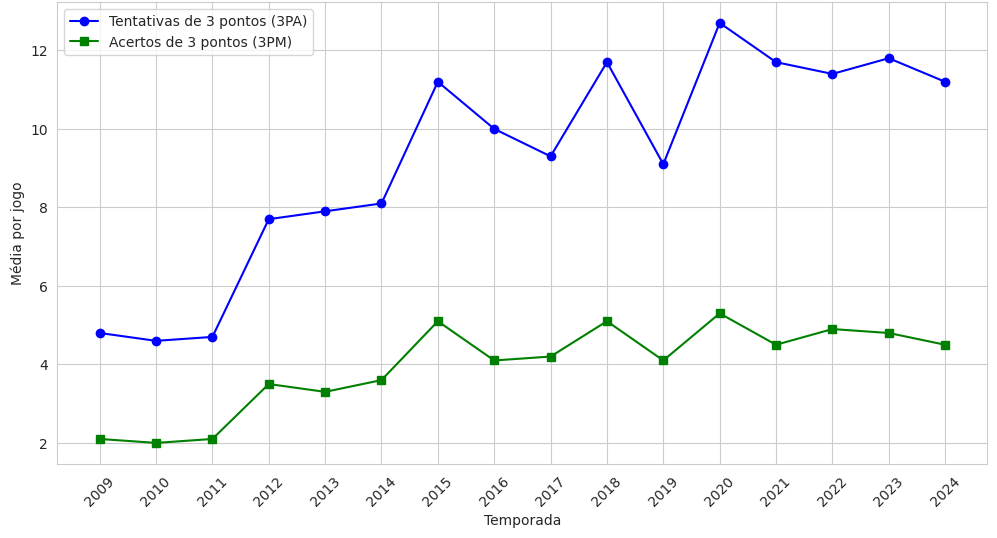
\includegraphics[width=\linewidth]{apendices/fig/14_IAA007_1.png}
\caption*{Fonte: O autor (2025).}
\end{figure}

\begin{figure}[H]
\centering
\caption{Porcentagem de Acerto em Arremessos de 3 Pontos de Stephen Curry}
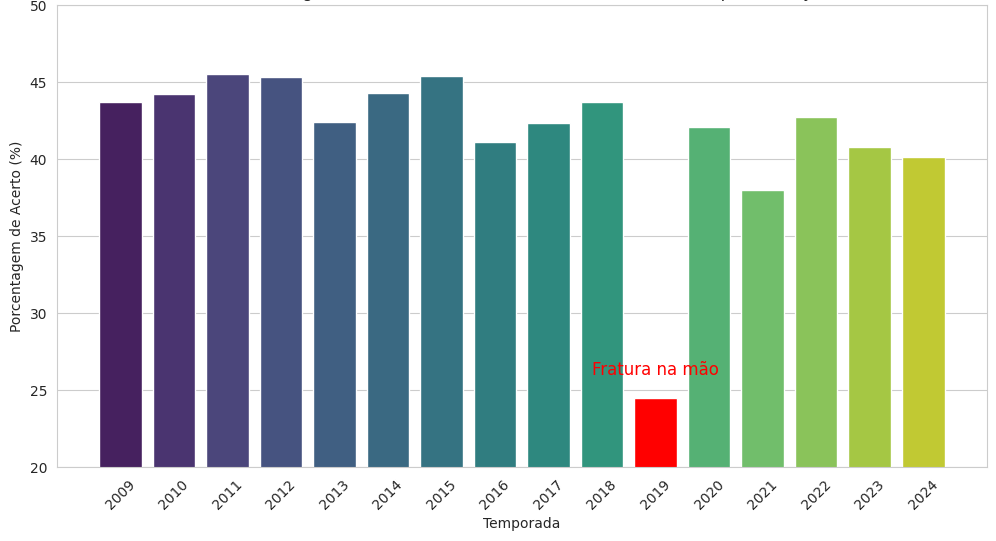
\includegraphics[width=\linewidth]{apendices/fig/14_IAA007_2.png}
\caption*{Fonte: O autor (2025).}
\end{figure}


\subsection*{\textbf{Código}}

\begin{lstlisting}[language=Python, style=input]
import pandas as pd
import matplotlib.pyplot as plt
import seaborn as sns

# Dados manuais do Curry na NBA (extraídos do Basketball Reference)
data = {
    'Temporada': ["2009", "2010", "2011", "2012", "2013", "2014", "2015", "2016", "2017", "2018", "2019", "2020", "2021", "2022", "2023", "2024"],
    '3PA': [4.8, 4.6, 4.7, 7.7, 7.9, 8.1, 11.2, 10.0, 9.3, 11.7, 9.1, 12.7, 11.7, 11.4, 11.8, 11.2],  # Tentativas de 3 pontos
    '3PM': [2.1, 2.0, 2.1, 3.5, 3.3, 3.6, 5.1, 4.1, 4.2, 5.1, 4.1, 5.3, 4.5, 4.9, 4.8, 4.5],  # Acertos de 3 pontos
    '3P%': [43.7, 44.2, 45.5, 45.3, 42.4, 44.3, 45.4, 41.1, 42.3, 43.7, 24.5, 42.1, 38.0, 42.7, 40.8, 40.1]  # Porcentagem de acerto
}

df = pd.DataFrame(data)

# estilo dos gráficos
sns.set_style("whitegrid")
plt.figure(figsize=(12, 6))

# Gráfico de evolução de tentativas e acertos de 3 pontos
plt.plot(df['Temporada'], df['3PA'], marker='o', linestyle='-', label='Tentativas de 3 pontos (3PA)', color='blue')
plt.plot(df['Temporada'], df['3PM'], marker='s', linestyle='-', label='Acertos de 3 pontos (3PM)', color='green')

# Destacando a queda em 2019
plt.annotate("Fratura na mão", xy=(10, 24.5), xytext=(8, 30),
             arrowprops=dict(facecolor='red', shrink=0.05), fontsize=12, color='red')

plt.xlabel("Temporada")
plt.ylabel("Média por jogo")
plt.title("Evolução dos Arremessos de 3 Pontos de Stephen Curry")
plt.legend()
plt.xticks(rotation=45)
plt.show()

# Gráfico de barras da porcentagem de acerto
plt.figure(figsize=(12, 6))
sns.barplot(x='Temporada', y='3P%', data=df, palette="viridis")

# destacando a queda em 2019
plt.text(10, 26, "Fratura na mão", fontsize=12, color='red', ha='center')
plt.bar(10, df['3P%'][10], color='red')

plt.xlabel("Temporada")
plt.ylabel("Porcentagem de Acerto (%)")
plt.title("Porcentagem de Acerto em Arremessos de 3 Pontos de Stephen Curry")
plt.xticks(rotation=45)
plt.ylim(20, 50)
plt.show()
\end{lstlisting}